
\subsection{Vista de distribución}

A partir de los componentes definidos en la vista de proceso,
se pueden extraer dos componentes principales importantes a la
hora de desplegar la aplicación.

\begin{figure}[H]
	\centering
	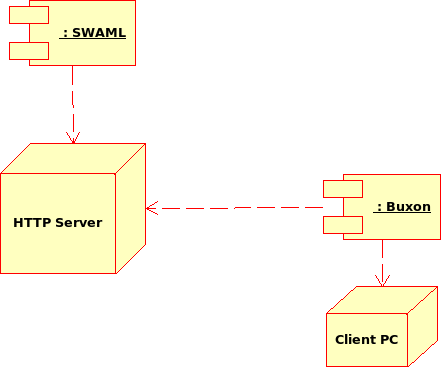
\includegraphics[width=12cm]{images/uml/despliegue.png}
	\caption{Diagrama de despliegue}
	\label{fig:uml:despliegue}
\end{figure}

Como se puede ver en el diagrama de despliegue descrito en la 
figura~\ref{fig:uml:despliegue}, el proceso principal de SWAML 
deberá ejecutarse en un servidor con capacidad para servir 
ficheros por HTTP. Buxon podrá, o no, estar en otro PC cliente
siempre y cuanto pueda establecer una conexión HTTP con el servidor
sobre el que han sido publicados los datos exportados por SWAML.